\documentclass[mathserif]{beamer}
\usetheme{Boadilla}
%\usepackage[francais]{babel}
\usepackage[utf8]{inputenc} % Uses the utf8 input encoding
\usepackage[T1]{fontenc} % Use 8-bit encoding that has 256 glyphs
\usepackage[style=authoryear,backend=biber]{biblatex}
\addbibresource{main.bib}
\usepackage{etoolbox}
\makeatletter
\patchcmd{\@@description}{\advance\beamer@descdefault by
  \labelsep}{\advance\beamer@descdefault by -1em}{}{}
\makeatother

\usepackage{calc}
\usepackage{xcolor}

\AtBeginSection[]
{
\setbeamercolor{section in toc}{fg=alerted text.fg}
\setbeamercolor{section in toc shaded}{bg=structure!20,fg=structure}
\setbeamertemplate{section in toc shaded}[default][100]
\begin{frame}<beamer>
  \frametitle{Outline}
  \tableofcontents[currentsection,hideallsubsections]
\end{frame}
}

\definecolor{myorange}{RGB}{180,90,0}

\definecolor{mygreen}{RGB}{70,140,0}

\newcommand{\mycite}[1]{{\color{mygreen} \small #1}}

\usepackage[nomath]{kpfonts}
\usepackage{eulervm}
%\usepackage{default}

\usepackage{amsthm}
\usepackage{amssymb}
\usepackage{xparse}
\usepackage{thmtools}
\usepackage{stackrel}

%shortcuts
\newcommand{\R}{\mathbb{R}}
\newcommand{\C}{\mathbb{C}}
\newcommand{\Z}{\mathbb{Z}}
\newcommand{\N}{\mathbb{N}}
\newcommand{\fii}{\varphi}
\newcommand{\dd}{\mathrm{d}}
\newcommand{\CP}{\mathbb{CP}}
\renewcommand{\S}{\mathbb{S}}
\DeclareMathOperator{\Sp}{Sp}
\DeclareMathOperator{\tr}{tr}
\DeclareMathOperator{\dist}{dist}

% theorems configuration

\makeatletter
\newtheoremstyle{indented}
{7pt} %vertical space before
{7pt} % vertical space after
{} %{\addtolength{\@totalleftmargin}{2.5em}
	%\addtolength{\linewidth}{-3.5em}
	%\parshape 1 3.5em \linewidth} %body font
{1.5em} %indent
{\bfseries} %header font
{.} %punctuation
{.5em} %horizontal space after header
{} %header specification

\theoremstyle{definition}

\newtheorem{defn}{Définition}[section]

\theoremstyle{plain}
%\newtheorem*{theorem*}{Theorem}

\newtheorem{thm}{Théorème}

\renewcommand{\thetheorem}{\Alph{theorem}}
\newenvironment{preuve}{
	\noindent \textbf{Proof. }}{\hfill $\square$\medskip\par}

\newtheorem{exemple}[defn]{Example}
\newtheorem{prop}[defn]{Proposition}
\newtheorem{corr}[defn]{Corollary}
\newtheorem{por}[defn]{Porisme}
\newtheorem{ex}[defn]{Example}
\newtheorem{lem}[defn]{Lemma}
\newtheorem{conj}{Conjecture}
\newtheorem{ax}{Axiom}  %Axioms have their own numerotation

\theoremstyle{definition}
\newtheorem{rem}[defn]{Remark} %remarks are not indented
\newtheorem{rems}[defn]{Remarks}

%--------------
% Mise en page mathématique
%--------------
\addtolength{\jot}{.2em}


\title{Szeg\H{o} kernels and Toeplitz operators}
\author{Alix Deleporte}
\date{February 14, 2020}
\institute[UZH]{Institut für Mathematik\\Universität Zürich}
\newcommand{\spline}{\hline}
\renewcommand{\arraystretch}{1.3}

\DeclareSourcemap{
  \maps[datatype=bibtex]{
    \map[overwrite=true]{
      \step[fieldsource=author,
            match=Deleporte,
            final]
      \step[fieldset=keywords, fieldvalue=Deleporte]
    }
  }
}
\begin{document}

\beamertemplatenavigationsymbolsempty

    \expandafter\def\expandafter\insertshorttitle\expandafter
       }%\insertframenumber}


\begin{frame}
	\titlepage
      \end{frame}

      \begin{frame}
  \frametitle{Positions}
  2016--2019: PhD (Strasbourg)

  \vfill

  2019: Postdoc (MSRI, Berkeley)

  \vfill

  2020--2???: Postdoc (Zürich)
\end{frame}

      \begin{frame}
        \frametitle{Outline}
        \begin{enumerate}
        \item Motivation: antiferromagnetic spin systems
          \begin{itemize}
          \item What are spin systems?
          \item Frustration in antiferromagnets
          \end{itemize}
        \item Toeplitz operators
          \begin{itemize}
            \item Definition of Toeplitz operators
            \item $L^2$ spaces of holomorphic functions and spectral
              gap
            \item Properties of Toeplitz operators
          \end{itemize}
        \item Localisation of low-energy states
          \begin{itemize}
          \item Localisation at principal order
          \item Subprincipal effects
          \item Applications to frustrated spin systems
          \end{itemize}
        \end{enumerate}
      \end{frame}

      \section{Motivation: antiferromagnetic spin systems}

\begin{frame}
  \frametitle{Introduction}
  \begin{itemize}
  \item<1-> {\bfseries spin systems}: models for magnetism in solids.
  \item<2-> {\bfseries classical spins}: one atom at site $i$
    $\rightsquigarrow$ one spin $s_i\in \S^2$.
  \item<3> Heisenberg antiferromagnet: Graph $G=(V,E)$,
    
    search the minima of the following energy:
    \[
      (s_i)_{i\in V}\mapsto\sum_{i\sim j}s_i\cdot s_j.
    \]
    Here $i\sim j$ when the atoms $i$ and $j$ are neighbours in $G$
    and $\cdot$ is the scalar product.
  \end{itemize}
\end{frame}

             \begin{frame}
         \frametitle{Introduction}
   \begin{center}
     \begin{picture}(50,100)
           \only<1>{\put(-125,-80){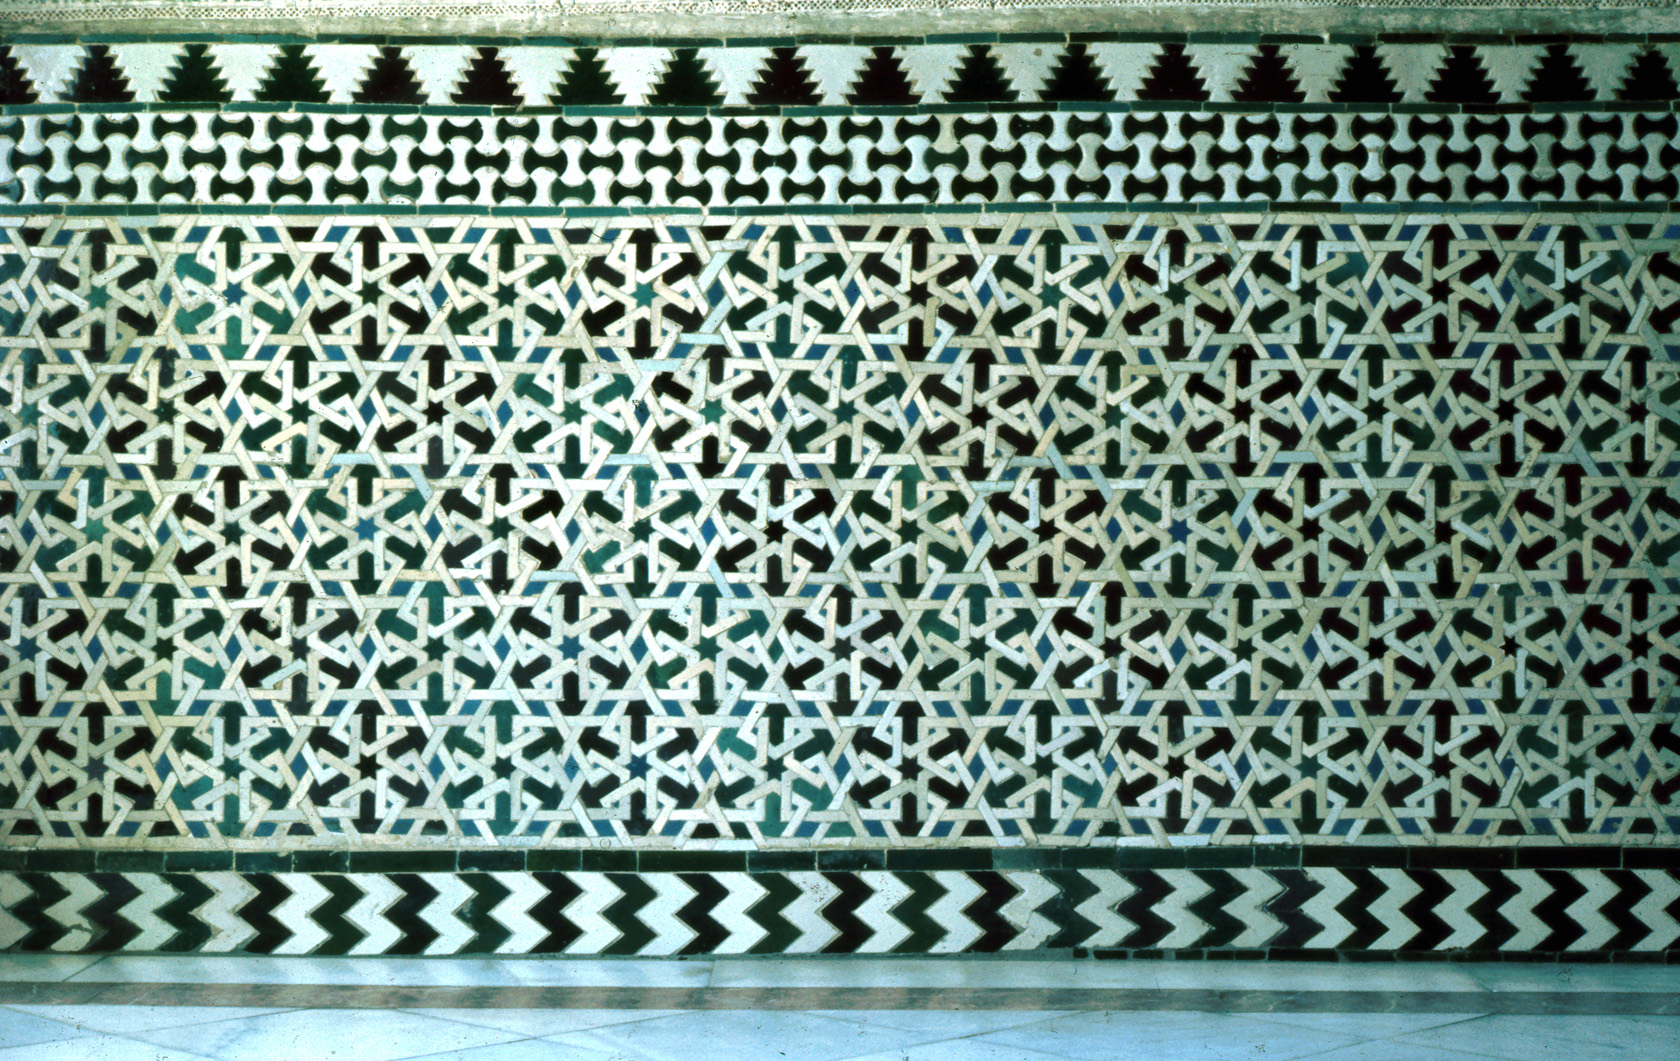
\includegraphics[scale=9]{Alcazar.png}}}
           \only<2>{\put(-125,-80){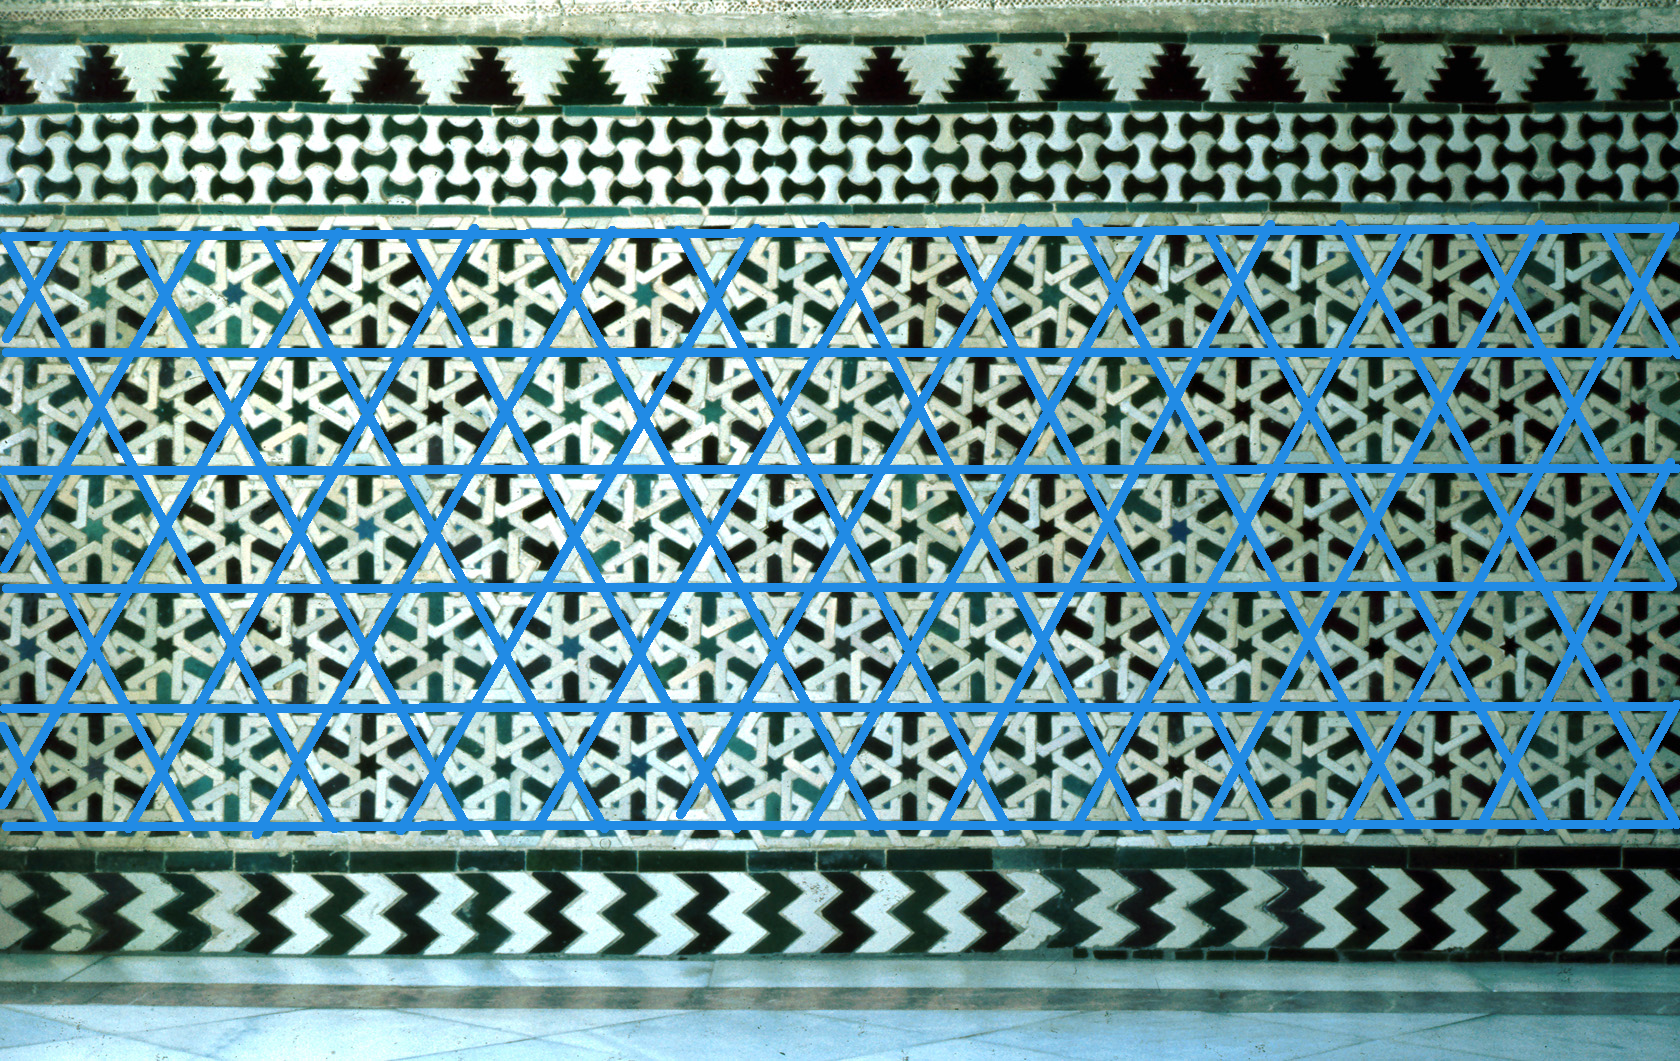
\includegraphics[scale=9]{Alcazar-Kagome.png}}}
           \only<3>{\put(-112,-80){\includegraphics[scale=0.32]{kagome-svg.png}}}
           \only<4>{\put(-112,-80){\includegraphics[scale=0.32]{kagome-spins-svg.png}}}
           \only<5>{\put(-112,-80){\includegraphics[scale=0.32]{kagome-spins-2-svg.png}}}
         \end{picture}
         \vspace{8em}

         Kagome lattice: \uncover<2->{appears in Zn$_2$Cu$_3$(OH)$_6$Cl$_2$ crystals.}
       \end{center}
     \end{frame}

     \begin{frame}\frametitle{Introduction}
       \begin{itemize}
       \item Quantum spin: self-adjoint matrices
         $S_x,S_y,S_z\in M_{N+1}(\C)$ \[[S_x,S_y]=\frac{2i}{N}S_z\qquad
           [S_y,S_z]=\frac{2i}{N}S_x\qquad [S_z,S_x]=\frac{2i}{N}S_y.\]
       \item Several spins $\rightarrow$ {\color{myorange} tensor product}.
         \[S_{x,i}=\underbrace{Id\otimes \cdots\otimes Id}_{i-1}\otimes S_x\otimes
           \underbrace{Id\otimes
             \cdots
             \otimes
             Id}_{d-i}.\]
         
       \item<2>
         Quantum
         energy
         (matrix
         of
         size
         $(N+1)^d$):
         \[
           \sum_{i\sim j}S_{i,x}S_{j,x}+S_{i,y}S_{j,y}+S_{i,z}S_{j,z}.\]
         
         
      \end{itemize}
    \end{frame}
    \begin{frame}
      \frametitle{Introduction}
      Quantum energy is a self-adjoint matrix $\Rightarrow$
      
      \hspace{1em}eigenvalues
      $\lambda_1\leq \lambda_2\leq \cdots\leq \lambda_{(N+1)^d}$

      \hspace{1em}and associated eigenvectors. \vspace{1em}
      
      Goal: {\color{myorange} qualitative study of eigenvectors} associated with
      $\lambda_1$ (ground states) or other small eigenvalues.
      
      \hfill
      
      \uncover<2>{Physics claim: {\color{myorange} quantum-classical
          correspondence} as $N\to +\infty$.
        
        \hfill
        
      Prediction \mycite{[Douçot-Simon 1998]}: lowest-energy eigenvectors concentrate on {\color{myorange} some} classical configurations.}
    \end{frame}
      \begin{frame}
        \frametitle{Introduction}
        Toeplitz quantization:
        \begin{itemize}
          \item treat $N\to +\infty$ as a semiclassical
       limit
     \item see eigenvectors above as sections over $(\S^2)^d$.
     \end{itemize}
     \uncover<2->{Questions:}
     \begin{itemize}
        \item<2-> Where does the ground state concentrate?
        \item<3> What is the decay speed outside the concentration set?
        \end{itemize}
      \end{frame}

      \begin{frame}
        \frametitle{Introduction}
        \setbeamercovered{transparent}
        {\footnotesize
        \begin{description}
        \item<1>[{[D. 2019]}] Alix Deleporte. “Low-Energy Spectrum of Toeplitz Operators: The Case
of Wells.” In: Journal of Spectral Theory 9 (2019).
\item<1-2> [{[D. 2020?]}] Alix Deleporte. “Low-Energy Spectrum of Toeplitz Operators with a
Miniwell.” In: Comm. Math. Phys, to appear.
\item<1>[{[D. 2018a++]}] Alix Deleporte. “Quantum Selection for Spin Systems.” In: arXiv
1808.00718 (2018).
\item<1>[{[D. 2018b++]}] Alix Deleporte. “The Bergman Kernel in Constant Curvature.” In:
arXiv 1812.06648 (2018).
\item<1-2>[{[D. 2018c++]}] Alix Deleporte. “Toeplitz Operators with Analytic Symbols.” In: arXiv
1812.07202 (2018).
\item<1>[{[D. 2019++]}] Alix Deleporte. “WKB Eigenmode Construction for Analytic Toeplitz
  Operators.” In: arXiv 1901.07215 (2019).
  \item<1-2>[{[D. 2020a++]}] Alix Deleporte. ``Fractional exponential
    decay in the forbidden region for Toeplitz operators.'' In: arXiv
    2001.07921 (2020).
    \item<1>[{[DV 2020b++]}] Alix Deleporte and San Vũ Ng\d{o}c. ``Uniform spectral asymptotics for semiclassical
wells on phase space loops''. In: arXiv 2002.00234 (2020).
        \end{description}}
    \end{frame}


    \AtBeginSection[]
{
\setbeamercolor{section in toc}{fg=alerted text.fg}
\setbeamercolor{section in toc shaded}{bg=structure!20,fg=structure}
\setbeamertemplate{section in toc shaded}[default][100]
\begin{frame}<beamer>
  \frametitle{Outline}
  \tableofcontents[currentsection,hideallsubsections]
\end{frame}
}

    
      \section{Toeplitz quantization}
      \begin{frame}
        \frametitle{Quantum-classical correspondence}
\begin{center}
	\begin{tabular}{|c|c|}
		\spline
	    Classical mechanics & Quantum mechanics\\
		\spline
		Symplectic manifold $M$ & Hilbert Space $H$\\ 
		\spline 
		Function $a\in C^{\infty}(M,\R)$ & Self-adjoint
                                                   operator $A\in L(H)$\\
		\spline
                Hamiltonien flow of $a$ & Flow of $e^{itA/\hbar}$\\
		\spline
		Poisson Bracket & Lie Bracket\\
		\spline
	\end{tabular}\end{center}\vspace{0em}
	\begin{itemize}
	\uncover<2>{\item Quantization : for a given classical
          model, how to construct an associated quantum
          model ?
	
	\item Semiclassics : the quantum model is $\hbar$-dependent. What
          can be said in the $\hbar\to 0$ limit ?}
	\end{itemize}
\end{frame}

\begin{frame}
  \frametitle{Toeplitz quantization}
  \begin{itemize}
  \item {\color{myorange} First step}: construct a sequence of
    orthogonal projectors $(S_N)_{N\in \N}$ acting on functions (or sections) on $M$.
    \item {\color{myorange} Second step}: associate to $a\in
      C^{\infty}(M,\R)$ the operator
      \begin{center}
\begin{array}{rcl}
 		T_N(a):Im(S_N)&\to & Im(S_N)\\
		u& \mapsto& S_N(fu\uncover).
 		\end{array}
\end{center}
\end{itemize}

\vfill

This procedure preserves self-adjointness and {\color{myorange}
  positivity}.

\vfill

\uncover<2>{
  Idea for $Im(S_N)$: consider spaces that are (over an open set $U$) of the form
  \[
    L^2(w)\cap \mathop{Hol}:=\left\{f:U\to \C \text{ holomorphic }, \int
    |f|^2w<+\infty\right\}.
  \]

  \vfill

  Semiclassical regime: $w=e^{N\Phi}$, with $N\to +\infty$.}
\end{frame}

\begin{frame}
  \frametitle{Spectral gap}
  $L^2(e^{N\Phi})\cap \mathop{Hol}$ is the kernel of
  $\overline{\partial}^*\overline{\partial}$ acting on $L^2(e^{N\Phi})$.

  \vfill

  The orthogonal projector $S_N:L^2(e^{N\Phi})\to L^2(e^{N\Phi})\cap \mathop{Hol}$  is well-behaved when
  $\overline{\partial}^*\overline{\partial}$ has a spectral
  gap.
  \begin{prop}[\mycite{Hörmander 1968}]
    If (and only if) $\partial\overline{\partial}\Phi$ is definite positive
    everywhere, then for some $c>0$, 
    \[
      \sigma(\overline{\partial}^*\overline{\partial})\subset
      \{0\}\cup [cN,+\infty).
      \]
    \end{prop}
  \end{frame}
  \begin{frame}
    \frametitle{Flat case}
    Standard case: on $\C^d\simeq \R^{2d}$, $\Phi$ is a positive
    definite quadratic form.
    \begin{itemize}
    \item $S_N$ is explicit: it has an integral kernel
      \[
        S_N(x,y)=cN^d\exp(-N\Psi(x,y)).
        \]
    \item One interpretation: projector onto the Lowest Landau Level
      of a constant magnetic field.
    \item $Im(S_N)$ is related to $L^2(\R^d)$ via a FBI transform.
    \end{itemize}
    {\color{myorange} Quantization check}: the bracket between
    Toeplitz operators is given by
    \[
      [T_N(f),T_N(g)]=\uncover<2>{\frac{i}{N}T_N(\{f,g\}_{\Phi})+O(N^{-2}),}\]
    \uncover<2>{where $\{\cdot,\cdot\}_{\Phi}$ is the Poisson bracket
      for the symplectic structure $\partial\overline{\partial}\Phi$.}
  \end{frame}

  \begin{frame}
    \frametitle{General case and gluing}
    On a compact manifold, gluing spaces of the form
    $L^2(e^{N\Phi})\cap \mathop{Hol}$ yields {\color{myorange}
      holomorphic sections of a line bundle} $L^{\otimes N}$ over $M$.

    \vfill

    Reciprocally, given a symplectic manifold $(M,\omega)$ and a
    compatible complex structure $J$ (Kähler), one can build $L$ by reading
    $\omega$ as $\partial\overline{\partial}\Phi$ in charts.

    \vfill

    If $M=\S^2$ with natural symplectic and complex structure, then
      \only<1>{\[T_N(\text{base coords})=\vphantom{\frac{N-2}{N}}\text{spin matrices}.\]}
  \only<2>{\[T_N(\S^2\ni (x,y,z)\mapsto x)=\frac{N-2}{N}S_x.\]}
\end{frame}
\begin{frame}
  \frametitle{Asymptotics of the Szeg\H{o} kernel}
 On $\C^d$, there holds $S_N(x,y)=cN^d\Psi^{\otimes
      N}(x,y)$, with
    $|\Psi|\asymp e^{-c\dist(x,y)^2}$.
    \uncover<2->{\begin{theorem}[\mycite{[Delin 1998]}]
        Let $M$ be a compact, {\color{myorange} $C^2$} Kähler manifold of
        dimension $d$. Then
        \[
          |S_N(x,y)|<CN^d\exp(-c\sqrt{N}\dist(x,y)).
        \]
      \end{theorem}
    }
    \uncover<3->{\begin{theorem}[\mycite{[Charles 2003]}]
        Suppose $M$ is {\color{myorange} $C^{\infty}$}. There exists a section
        $\Psi$ and a sequence of functions $(s_k)_{k\geq 0}$ on
        $M\times M$ such that
      \[
        S_N(x,y)=N^d\Psi^{\otimes
          N}(x,y)(s_0+N^{-1}s_1+\cdots)(x,y)+O(N^{-\infty}).
      \]
      Here, for some $c>0$, $
        |\Psi(x,y)|\leq e^{-c\dist(x,y)^2}.$
      \end{theorem}

      If $M$ is {\color{myorange} analytic}, $S_N$ is known up to
    $O(e^{-cN})$. \mycite{[\underline{D. 2018c++},
        Rouby-Vũ \vspace{-0.6em}\begin{flushright}Ng\d{o}c-Sjöstrand 2018++]\end{flushright}}
    }
  \end{frame}

  \begin{frame}
    \frametitle{Calculus of Toeplitz operators}
    Asymptotics of the Szeg\H{o} kernel $\Rightarrow$ composition and
    inversion of Toeplitz operators.

    \begin{theorem}[{\mycite{[Schlichenmaier 2000]}}]Let $M$ be smooth. Let $a$ and $b$ be
      smooth real-valued functions on $M$. Then there exists a sequence $(c_k)_{k\geq
        0}\in (C^{\infty}(M,\R))^{\N}$ such that
      \[
        T_N(a)T_N(b)=T_N(c_0+N^{-1}c_1+\cdots)+O(N^{-\infty}).
        \]

        If $a$ does not vanish, then there exists a sequence
        $(d_k)_{k\geq 0}\in (C^{\infty}(M,\R))^{\N}$ such that
        \[
          T_N(a)T_N(d_0+N^{-1}d_1+\cdots)=S_N+O(N^{-\infty}).
          \]
        \end{theorem}
        Calculus in analytic regularity (up to $O(e^{-cN})$):
        \mycite{[\underline{D. 2018c++}]}.
  \end{frame}

\begin{frame}
  \frametitle{Toeplitz operators versus $\Psi$DOs}
  \begin{itemize}
  \item In the case $M=\C^d, \Phi=|z|^2$, an FBI transform $\mathcal{B}_N$ conjugates $Im(S_N)$ and
    $L^2(\R^n)$.
  \uncover<2->{
  \item With {\color{myorange} $g_N=(N/\pi)^ne^{-N|z|^2}$} one has
    \[
      \mathcal{B}_N^{-1}T_N(f)\mathcal{B}_N=Op_W^{N^{-1}}(f*g_N).
    \]\vspace{-2em}}
\uncover<3->{\item Equivalence between Toeplitz and $\Psi$DO
  calculus in the $C^{\infty}$ class.}
\uncover<4>{\item Toeplitz quantization is formulated {\color{myorange} directly in
  phase space}, it is {\color{myorange} positive} and
{\color{myorange} better behaved for rough symbols}.}

  \end{itemize}
\end{frame}




\section{Localisation of low-energy states}

\subsection{Localisation at the classical minimal set}
\begin{frame}
  \frametitle{Speed of localisation}
 For $N\in \N$, let $u_N$ be a normalised eigenvector associated with
 the smallest eigenvalue of $T_N(f)$. Let $Z=\mathop{argmin}(f)$.
  \begin{theorem}[\mycite{[Charles 2000]}]
  If f is {\color{myorange}smooth} and $U\subset M$ is at positive distance from $Z$, then \[\int_{U}|u_N|^2=O(N^{-\infty}).\]\vspace{-1.2em}
\end{theorem}
\uncover<2>{
\begin{theorem}[\mycite{[\underline{D. 2018c++}]}]
If f is {\color{myorange}real-analytic} then\vspace{-1em}
      \[
        \int_{U}|u_N|^2=O(e^{-cN}).%\vspace{-0.5em}
      \]
    \end{theorem}
  }

  \begin{itemize}
  \item Tool: calculus of Toeplitz operators
  \item  Context: fixed manifold, $N\to +\infty$.
  \end{itemize}
\end{frame}

  \begin{frame}
  \frametitle{Speed of localisation -- improved}
  \begin{theorem}[\mycite{[\underline{D. 2020a++}]}]
    If $f$ is {\color{myorange} $L^{\infty}$}, $M$ is
    {\color{myorange} $C^{1,1}$} and $U\subset M$ is at
    positive distance from $Z$, then
    \[
      \int_U |u_N|^2=O(e^{-cN^{\frac 14}}).
      \]
    \end{theorem}
    If $f$ or $M$ is more regular, we get up to $O(e^{-cN^{-\frac 12}})$.

    \begin{itemize}
      \item Tool: off-diagonal decay of the projector.
      \item Context: fixed manifold, $N\to +\infty$.
      \end{itemize}
    \end{frame}

    \begin{frame}
      \frametitle{Speed of localisation -- uniformity in $d$}
      Case where $f$ is a ``spin system'' on $(\S^2)^d$.
      \begin{theorem}
        [\mycite{[\underline{D. 2020a++}]}]
        If $T_N(f)u=\lambda u$, then with
        \[
          U=\{|f-\lambda|\geq C(f)N^{-\frac 14}d^{\frac 34}\},
        \]
        one has
        \[
          \int_U
          e^{c(f)\frac{\sqrt{N}\dist(\cdot,U)}{\sqrt{d}}}|u|^2\leq
          C(f)\|u\|_2^2.
          \]
        \end{theorem}
        Here, $C(f)$ is {\color{myorange} independent on $d,N,\lambda$}.

        Application: quantum free energy $f_Q$ versus classical free
        energy $f_C$: if $\beta<c(f)d$, then
        \[
          |f_Q(\beta,d)-f_C(\beta,d)|\leq C(f)N^{-\frac 12}.
          \]
    \end{frame}


\subsection{Subprincipal effects on localisation}

\begin{frame}
  \frametitle{Characteristic value}
  \begin{itemize}
  \item For $x\in Z$ a minimal point for $f$, we construct $\mu(x)$
    associated with the Hessian of $f$ at $x$.
  \item<2-> {\color{myorange} Quantum selection}: the ground states of $T_N(f)$
    concentrate only on the subset $Z_{\mu}$ of $Z$ where also $\mu$ is minimal.
  \end{itemize}
  
  \uncover<3>{\begin{itemize}
    \item case of a Schrödinger operator $-\hbar^2\Delta+V$
      \mycite{[Helffer-Sjöstrand 1986]}, where
      \begin{itemize}
      \item $V$ vanishes on a smooth submanifold $Z$
      \item Its transverse Hessian is nondegenerate on $Z$.
      \end{itemize}
    \item ``Magnetic bottles'' \mycite{[Helffer-Morame 2001,
        Helffer-Kordyukov 2009, ...]}
    \end{itemize}
    }

\end{frame}

\begin{frame}
  \frametitle{Subprincipal localisation}
  Quantum selection in general for Toeplitz operators:
  \begin{theorem}[\mycite{[\underline{D. 2020?}]}]
    Let $M$ be smooth, let $f\in C^{\infty}(M,\R)$ and let $Z_{\mu}$ and
    $(u_N)_{N\geq 1}$ be as above.

    For all $U\subset M$ at positive distance from $Z_{\mu}$, one has
    \[
      \int_U
      |u_N|^2=O(N^{-\infty}).
      \]
    \end{theorem}

    \begin{itemize}
      \item If $Z$ has a simple structure near $Z_{\mu}$, one can build
        quasimodes.
        \item Tools: Calculus of Toeplitz operators, cutting the phase
          space.
        \item Context: fixed manifold, $M\to +\infty$.\
        \end{itemize}
        
    
\end{frame}

 \subsection{Future work}
\begin{frame}
  \frametitle{Perspectives}
    \begin{itemize}
    \item Better estimates for $d \to +\infty$, incorporate
      subprincipal terms (``linear spin wave theory'')
    \item Low-energy dynamics.
    \item Geodesics in the space of Kähler metrics
    \item Non self-adjoint operators with analytic symbols (Scottish flag).
    \end{itemize}
  \end{frame}

  \begin{frame}
    \frametitle{Thanks}
    \centering 
    {\Large Thanks for your attention!}
  \end{frame}

\end{document}
%%% Local Variables:
%%% mode: latex
%%% TeX-master: t
%%% End:
